% !TeX program = xelatex
\documentclass{nwputhesis}
\usepackage{gbt7714}
\usepackage{fancyhdr}
\usepackage{hyperref}
\usepackage{listings}
\lstset{basicstyle=\ttfamily}
\begin{document}

% 生成封面, 使用\maketitle 
% 该封面不同学院要求可能不同,如有需要,请在cls文件中自行修改
\maketitle

\newpage
% 目录
\makecontent
\iffalse
    \makefigcontent
    \maketabcontent
\fi
% 正文
\maketext
\fancyfoot[C]{\thepage}
\pagestyle{fancy}
\section{总览}
\subsection{全文预览}
123
\makespace
\section{实习目标}
\subsection{学习方向及目标}
学习现在先进的计算机视觉(Computer Vision)以及图形学与AI结合的模型如\textbf{Neural Radiance Fields}(神经辐射场,简称NeRF),
\textbf{3D Gaussian Splatting}(3D高斯溅射,简称3dgs),以及\textbf{YOLO}(全称You Only Look Once),同时理解各个模型的实现原理。
\subsection{期望}
\begin{itemize}
    \item 完成搭建尽可能多的AI模型,配置其环境,并完成训练其预设数据库。
    \item 学习并理解各个模型的实现原理。
    \item 自己制作数据并通过基于AI的三维重建制作模型。
\end{itemize}
\makespace
\section{Yolo V5}
\subsection{模型简介}
\textbf{Yolo}(You Only Look Once)是一种单阶段目标检测算法,即仅需要 “看” 一次就可以识别出图片中物体的class类别和边界框。\textbf{Yolov5}是由
\textbf{Alexey Bochkovskiy}等人在\textbf{YOLO}系列算法的基础上进行改进和优化而开发的,使其性能与精度都得到了极大的提升。
\subsection{模型环境配置}
\noindent 于CUDA 10.2 基础下:
\begin{itemize}
    \item Python = 3.8.19
    \item torch = 2.3
    \item torchvision = 0.18.0
    \item gitpython = 2.40.1
    \item opencv-python = 4.9.0.80
    \item matplotlib = 3.7.5
    \item pandas = 2.0.3
\end{itemize}
模型从\underline{https://github.com/ultralytics/yolov5.git}克隆下来,然后在本地进行配置。

\subsection{模型训练}
\indent 模型训练是在\textbf{train.py}文件中进行的,训练时可以同时输入\textbf{data}\footnote{文件中包含了训练集和验证集的路径,
以及所有的标注种类}、\textbf{cfg}\footnote{文件中包含了模型的参数,如学习率、batch size等}和\textbf{weight}\footnote{文件
中包含了预训练模型的权重}文件;或是\textbf{epochs}\footnote{训练的次数}和\textbf{batch size}\footnote{每次训练的图片数量}。
\\
如下图:
\begin{figure}[H]
    \centering
    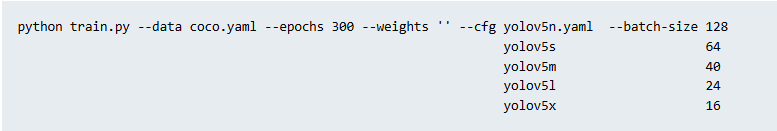
\includegraphics[width=0.8\textwidth]{picture/2.png}
    \caption{YOLOv5目标检测模型的训练命令}
\end{figure}
\subsection{测试自己制作的数据集}
从网上找寻了30张宝可梦的图片,然后通过\textbf{labelImg}工具\footnote{LabelImg 是一个开源的图像标注工具,用于创建图像数据集时
标记图像中的对象边界框}标注这些图片中比较常见的宝可梦,如皮卡丘、杰尼龟等,然后将这些图片和标注文件放入到一个文件夹中。最后通过
\textbf{YOLOv5}模型进行训练,得到了一个可以识别这些宝可梦的模型,因为数据集比较小,所以模型的识别率不是很高。
\\
\indent 训练结果示例:
\begin{figure}[H]
    \centering
    
\includegraphics[width=0.8\textwidth]{picture/3.png}
    \caption{YOLOv5目标检测模型的训练结果}
\end{figure}
\makespace
\subsection{实现原理}
\textbf{YOLOv5}首先会在输入端中将输入图片进行预处理,图像大小调整为模型所需的大小,进行归一化操作,及将像素值缩放到0到1之间。\\
\indent 然后将图片输入到\textbf{backbone网络}\footnote{backbone网络是一个特征提取网络,用于提取图片的特征}中,
\textbf{backbone}网络会将图片的特征提取出来,然后将这些特征输入到\textbf{neck网络}\footnote{neck网络是一个特征融合网络,用
于将不同层次的特征进行融合}中,\textbf{neck网络}会将不同层次的特征进行融合,然后将这些特征输入到\textbf{head网络}
\footnote{head网络是一个预测网络,用于预测图片中的物体}中,\textbf{head网络}会将图片中的物体进行预测,得到物体的类别和边界框。
\\
\indent 下图为\textbf{YOLOv5}的网络结构:
\footnote{CPL:由卷积Conv+批量归一化BN+激活函数Leaky Relu组成,用于在特征提取的过程中增加网络的信息传递能力。CPL通过在不同阶段的特征图之间进行部分连接,使得网络可以更充分地利用低级和高级特征,从而提高模型的性能。}
\footnote{CSP1:由CBL模块、Res uint模块以及卷积层Concat组成。CSP1是CPL的一种变体,它在CPL的基础上引入了跨阶段的残差连接,以进一步增强网络的信息传递能力。CSP1可以有效地减少网络中的计算量,提高模型的效率。}
\footnote{CSP2:不再使用Res unit,由卷积层CBL模块Concat组成。CSP2引入了路径重排的技术,以重新排列网络中的路径,使得前向和后向传播之间的信息流更加平滑和高效。这种路径重排有助于减少网络中的计算量,提高模型的速度和效率。CSP2同样也进行了路径融合(Path Fusion),即在不同路径之间进行信息融合,以使网络可以更充分地利用低级和高级特征。这种路径融合有助于提高模型对目标的检测和识别能力。CSP1也具有类似的路径融合机制。}
\footnote{SPP是一种用于空间金字塔池化的技术,它能够在不同尺度下提取图像的局部特征。SPP在YOLOv5中用于提取特征图的空间信息,从而使得模型可以更好地检测不同尺度和大小的目标。}
\footnote{Focus:对图像进行切片后再Concat}
\footnote{上采样:利用元素复制扩充的方法使得特征图尺寸扩大,例如线性插值。}
\footnote{Concat:张量拼接,会扩充两个张量的维度,实现多尺度特征融合。}
\begin{figure}[H]
    \centering
    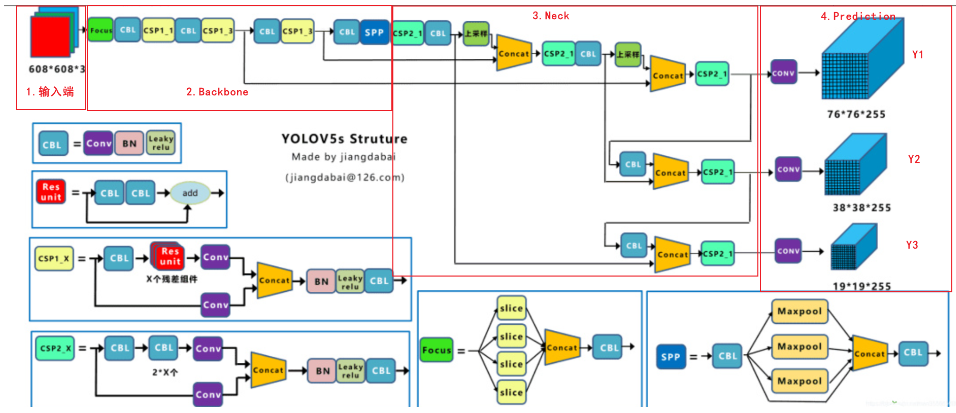
\includegraphics[width=0.8\textwidth]{picture/4.png}
    \caption{YOLOv5的网络结构}
\end{figure}
\makespace
\section{NeRF}
\subsection{模型简介}
\textbf{NeRF}(Neural Radiance Fields)是一种用于三维重建的深度学习模型,它可以从二维图像中重建出高质量的三维场景。
\textbf{NeRF}的核心思想是利用神经网络来建模场景中每个空间点的辐射亮度和密度,从而实现对场景的准确重建。
\subsection{模型环境配置}
\noindent 于CUDA 10.2 基础下:
\begin{itemize}
    \item Python = 3.7.1
    \item cudatoolkit = 10.0.130
    \item tensorflow = 1.14.0
    \item numpy = 1.21.5
    \item imageio = 2.193
    \item configargparse = 1.4
\end{itemize}
模型从\underline{https://github.com/bmild/nerf.git}克隆下来,然后在本地进行配置。

\subsection{模型训练}
\indent 模型训练是在\underline{run\_nerf.py}文件中进行的,需要同时输入配置文件的的相对路径,配置文件中包含了
\textbf{实验名称}(expname),\textbf{基础目录}(basedir),\textbf{数据集路径}(datadir),\textbf{数据集类型}
(dataset\_type)\textbf{采样参数}、\textbf{使用视角方向信息}等模型训练和数据配置信息。

\subsection{训练结果}
先在730显卡的电脑上配置环境并尝试训练,但因预计训练结束时间要20左右,后改为在3080显卡的电脑上
重新配置环境。在重新配置环境时遇到一些版本冲突的问题,因为3080显卡的电脑上的CUDA版本是12.3,
不能与原配置的\textbf{tensorflow}版本1.14.0兼容,所以需要重新配置环境。最后在3080显卡的电脑上重新配置
环境并训练,但最后的预计训练结束时间人在一天左右,所以在\textbf{github}上找到了另外一个模型
\textbf{NeRF Pytorch}(详情见\hyperlink{section 5}{第5章 NeRF Pytorch})。
\makespace
\subsection{实现原理}
\subsubsection{NeRF的核心思想}
简单一点理解可以把\textbf{NeRF}看作是用\textbf{深度全连接神经网络}(deep fully-connected neural network,MLP)
\footnote{通常被称为多层感知机(multilayer perceptron)或MLP,没有卷积层(convolutional layers),由全连接层
(fully connected layer)和激活函数(activation function)组成}去学习并训练一个静态3D场景,实现复杂场景的任意新视角
合成(渲染)。NeRF的核心思想是将静态场景表示为5D函数,即每个\textbf{空间点x}$(x,y,z)$和\textbf{方向d}$(\theta
\footnote{极角(Polar Angle),通常的取值范围是0到π之间,通常表示从参考方向(通常是参考坐标系的正方向)到目标向量(或
目标位置)的角度,简单一点可以理解为与z轴的夹角}, \phi\footnote{方位角(Azimuthal Angle),通常的取值范围是0到2π之间,
通常表示目标向量在参考平面上投影与参考方向的夹角,简单一点可以理解为在xy平面上与x轴的夹角})$都对应一个
\textbf{颜色}(RGB)和\textbf{密度}$(\sigma)$。
\subsubsection{输入模型前的准备}
\textbf{NeRF}的输入是一条被5D函数(即即每个空间点x$(x,y,z)$和方向d$(\theta,\phi)$代表的射线,输出是射线上每个点的颜
色和密度。其中方向d$(\theta,\phi)$,在进入模型前将先会被展开成\textbf{三维笛卡尔坐标}(3D Cartesian)系下的单位向量
\(\vec{u}\)。这种单位向量可以用来表示一个方向,它有着确定的$x,y,z$三个分量,记为$(ux, uy, uz)$。由于是单位向量,所以
这三个分量要满足(公式2.1):
\begin{equation}
    \begin{aligned}
        u_x^2 + u_y^2 + u_z^2 = 1
        \captionsetup{labelformat=default}
    \end{aligned}
\end{equation}
$(ux, uy, uz)$具体的计算公式如下(公式2-2):
\begin{equation}
    \begin{aligned}
        u_x &= \sin(\theta)\cos(\phi)\\
        u_y &= \sin(\theta)\sin(\phi)\\
        u_z &= \cos(\theta)
    \end{aligned}
\end{equation}
\indent
在进入模型前, 通常还会先将空间点$x(x,y,z)$和方向$d(ux, uy, uz)$通过\textbf{位置编码}(positional encoding)
\footnote{位置编码是一种将空间位置信息映射到更高维的空间中的技术,它可以帮助模型更好地理解空间位置信息,从而提高模型的性
能。}映射到更高维的周期性函数空间\footnote{周期性函数空间是指由周期函数构成的函数空间。一个周期性函数$f(x)$是指满
足$f(x+T) = f(x)$的函数,其中$T$是一个常数,称为周期。}中,以增加模型的表达能力。转换公式示例如下(公式2-3):
\begin{equation}
    \begin{aligned}
        r(x) &= (\sin(2^0\pi x), \cos(2^0\pi x), \sin(2^1\pi x), \cos(2^1\pi x), \cdots, \sin(2^{L-1}\pi x), \cos(2^{L-1}\pi x))
    \end{aligned}
\end{equation}
\indent
及将一个一维向量$x$映射到一个$2L$维的向量,在论文中作者对空间点$x(x,y,z)$转换成了60维的向量,即$L=10$,$3 \times 2L(L=10) = 60$,
同时将方向d从3维$(ux, uy, uz)$转换成了24维的向量,即$L=4$,$3 \times 2L(L=4) = 24$。
(详情见\hyperlink{图2-5}{图2-5})。下图为论文实验时使用位置编码和不使用位置编码的对比图:
\begin{figure}[H]
    \centering
    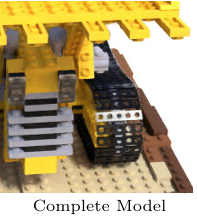
\includegraphics[width=0.4\textwidth]{picture/6.png}
    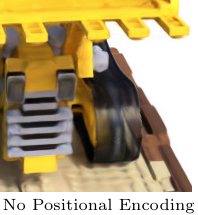
\includegraphics[width=0.4\textwidth]{picture/7.png}
    \caption{使用位置编码和不使用位置编码的对比图}
\end{figure}
\indent
从上图中可以看出在使用了位置编码后,模型在细节的表达中会更好,尤其是在凹凸不平的地方,而不使用位置编码的模型在这些地方会变得模糊。\\
\\
\indent
在实际使用位置编码时除了上述公式中的$2L$维向量外,有时还会加上一个维度为1的向量和表示其本身的向量进行拼接成为$2L+2$维的向量(论文的实验中
并未使用$2L+2$维的向量,这里仅仅只是补充说明),这两个向量的加入可以帮助模型更好的学习低频平滑部分,同时提高模型的灵活性。加入后的新向量
如下(公式2-4):
\begin{equation}
    \begin{aligned}
        r(x) &= (\sin(2^0\pi x), \cos(2^0\pi x), \sin(2^1\pi x), \cos(2^1\pi x), \cdots, \sin(2^{L-1}\pi x), \cos(2^{L-1}\pi x), x, 1)
    \end{aligned}
\end{equation}

\subsubsection{模型设计与输出}
空间点$x(x,y,z)$通过位置编码升维过后的高维向量会先进入\textbf{深度全连接神经网络}(MLP)中,在经过多层的
\textbf{全连接层}和\textbf{激活函数}(Activation Function)\footnote{激活函数的作用是在神经网络中引入非线性因素
,使得整个网络由线性变换的组合升级为非线性变换的组合,从而能够拟合更加复杂的映射函数。没有激活函数,即使是深层网络
,最终的输出也只能是输入的线性组合,表达能力是有限的。}后,最后输出密度($\sigma$)和 一个维度和之前全连接层维度
相同的中间特征向量,中间特征会和三维方向向量d通过位置编码升维过后的高维向量一起输入到额外的全连接层中去预测颜色
(RGB)。示例如下图:
\hypertarget{图2-5}{}
\begin{figure}[H]
    \centering
    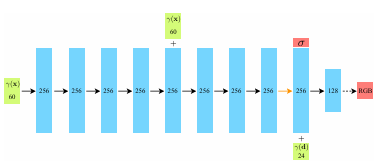
\includegraphics[width=0.8\textwidth]{picture/5.png}
    \caption{NeRF中的MLP结构示例}
\end{figure}
在论文中(如上图)作者使用了8层的全连接层,每层的隐藏单元数为256,激活函数为\textbf{ReLU}(
Rectified Linear Unit),空间点$x(x,y,z)$在进入这个8层的全连接层后输出了密度($\sigma$)和一个维度为256的中间
特征向量。这个中间特征向量和和方向d一起进入一层额外的全连接层中去预测颜色(RGB),这个额外的全连接层包含了激活
函数ReLU和128个隐藏单元。\\
\indent
其中第一个全连接层的权重矩阵大小为$60 \times 256$,及60维的输入向量在进入全连接层后会变成256维的向量,运算公式如下(公式2-5):
\begin{equation}
    \begin{aligned}
        x &= \begin{bmatrix}
            x_1 & x_2 & ... & x_{59} & x_{60}
        \end{bmatrix}
        \\
        w &=
            \begin{bmatrix}
                    w_{1,1} & w_{1,2} & ... & w_{1,255} & w_{1,256}\\
                    w_{2,1} & w_{2,2} & ... & w_{2,255} & w_{2,256}\\
                    \vdots & \vdots & \vdots & \vdots & \vdots\\
                    w_{59,1} & w_{59,2} & ... & w_{59,255} & w_{59,256}\\
                    w_{60,1} & w_{60,2} & ... & w_{60,255} & w_{60,256}\\
            \end{bmatrix}
        \\
        x \times w &= y = \begin{bmatrix}
            y_1 & y_2 & ... & y_{255} & y_{256}
        \end{bmatrix}
        \\
        \text{where: \space} y_n &= x_1w_{1,n} + x_2w_{2,n} + ... + x_{59}w_{59,n} + x_{60}w_{60,n} + b_n 
    \end{aligned}
\end{equation}
\indent
第二到第五个全连接层的权重矩阵大小为$256 \times 256$。但在进入第6个全连接层之前,又输入了一个与初始输入相同的60维向量,所以第6个全连接层
的输入为一个316维的向量,输出为256维的向量,所以第六个全连接层的权重矩阵大小为$316 \times 256$。第七与第八个全连接层的权重矩阵大小为
$256 \times 256$。第9个全连接层在输入时除了256维的中间向量以外还输出了密度$(\sigma)$,及输出了一个257维的向量,所以第九个全连接层的权重
矩阵大小为$256 \times 257$。第十个全连接层的输入除了刚刚提到的256维的中间向量以外,24维的经过位置编码升维过后的24维方向向量也进入了模型
所以第十个全连接层的输入是280维的向量,且输出为128维的向量,所以第十个全连接层的权重矩阵大小为$280 \times 128$。最后这个128维向量在进入
一个$128 \times 3$的权重矩阵后输出了3维的颜色(RGB)。
\\
\indent
上文还提到了,在全连接层中同时也用到了ReLU(Rectified Linear Unit)这种激活函数,ReLU激活函数的公式如下(公式2-6):
\begin{equation}
    \begin{aligned}
        f(x) = \max(0,x)
    \end{aligned}
\end{equation}
表面上来看ReLU只是简单的将小于0的值截为0,但实际上它引入了一个分段线性的非线性函数:
\begin{enumerate}
    \item 当输入大于0时,ReLU(x)=0,输出是一个常量
    \item 当输入小于0时,ReLU(x)=x,输出与输入是线性关系
\end{enumerate}
这两个分段线性区域的接合点$(x=0)$引入了一个折线的不连续点,使得整个映射函数不再是单纯的线性方程,而具有了非线性的性质。如下图(图2-6):
\begin{figure}[H]
    \centering
    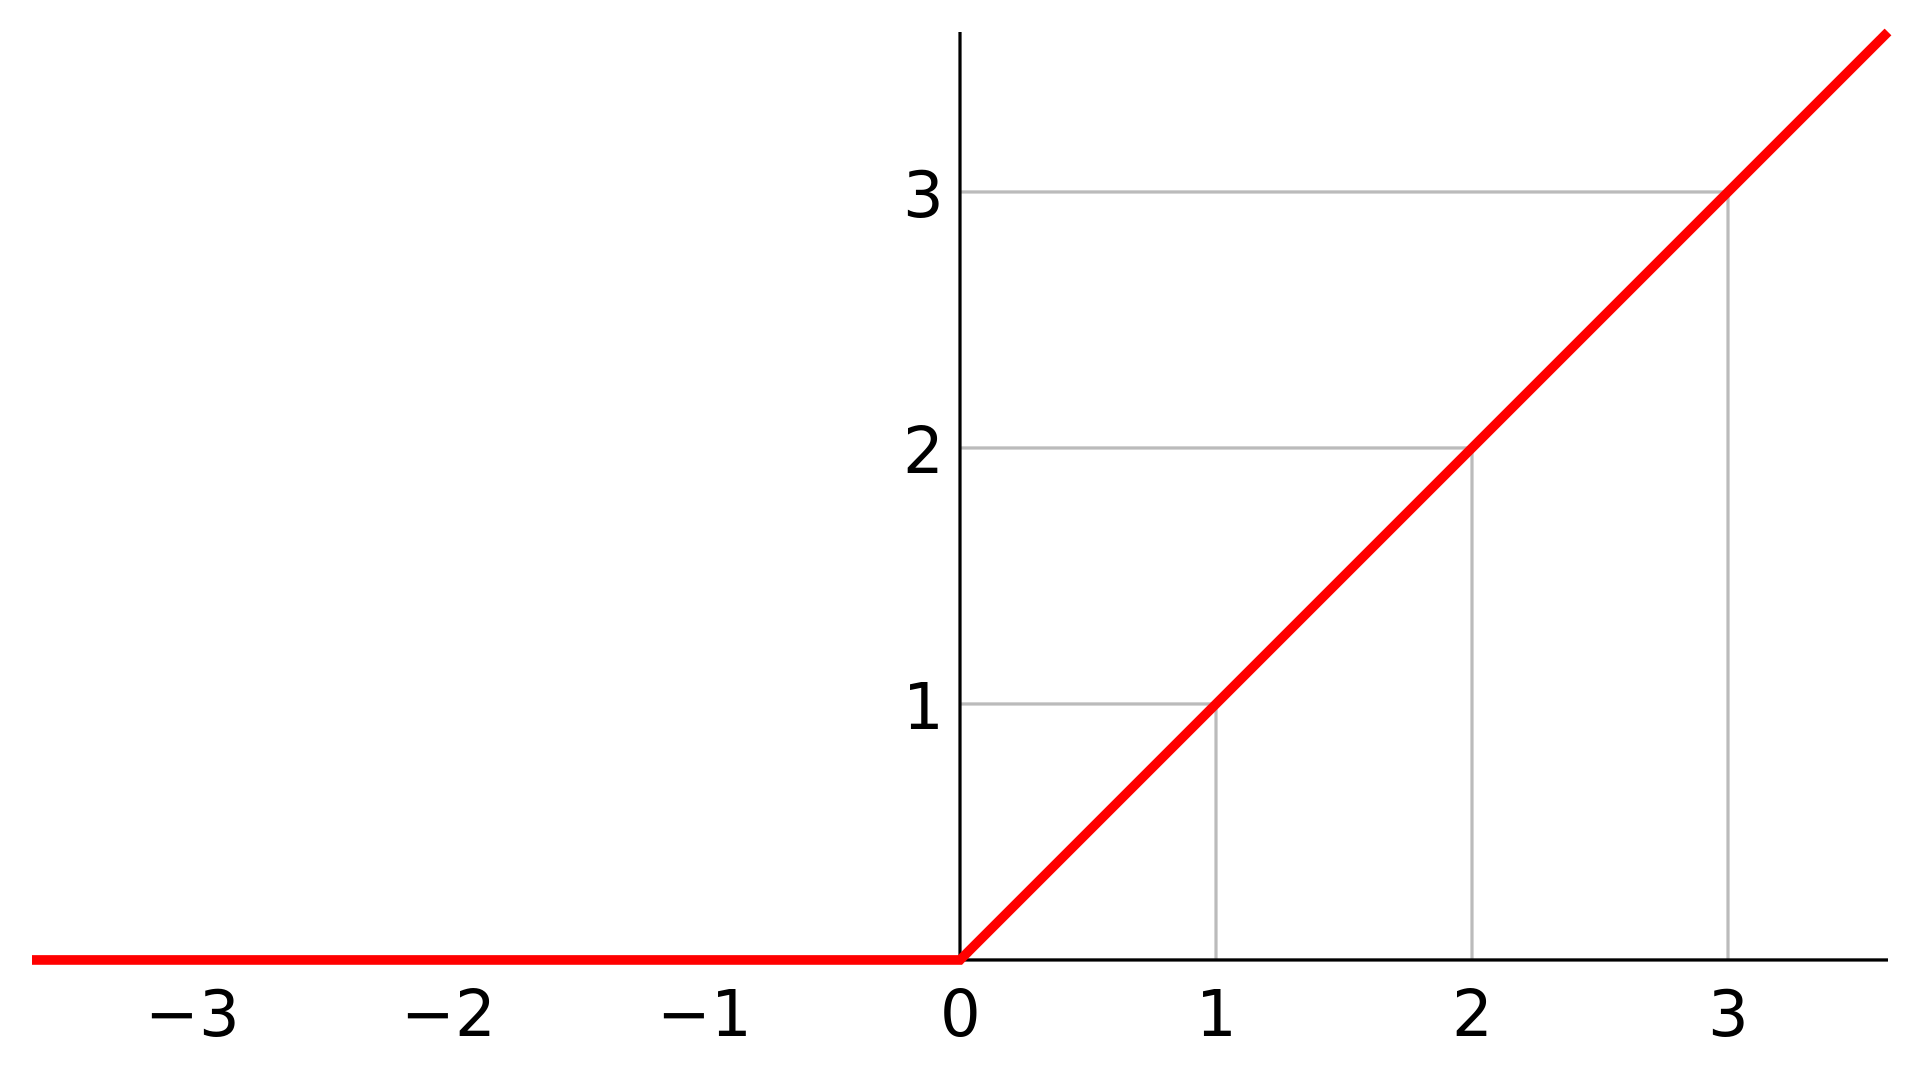
\includegraphics[width=0.8\textwidth]{picture/8.png}
    \caption{ReLU激活函数示例}
\end{figure}
\subsubsection{渲染(Rendering)}
\textbf{NeRF}使用了经典的\textbf{体积渲染}(Volume Rendering)技术,即通过对每个射线上的点进行采样,然后将采样点的颜色和密度进行加权平均,从而得到整个射
线的颜色。相机射线$r(t) = o + td$(其中$o$是射线的起点,$d$是射线的方向向量,$t$是参数)在近端和远端界
限$t_n$与$t_f$之间的预期颜色$C(r)$可表示为(公式2-7):
\begin{equation}
    \begin{aligned}
        C(r) &= \int_{t_n}^{t_f} T(t)\sigma(r(t))c(r(t),d)dt
    \end{aligned}
\end{equation}
\indent
其中$\sigma$是之前在模型中预测的密度,$\sigma(r(t))$是沿着光线r在位置t处的体密度值,因为$r(t)$是一个点在空间中
的位置,所以$\sigma(r(t))$也可以更简单的理解为在点$(x,y,z)$在密度。$c(r(t),d)$是是沿着光线r在位置t处的颜色
其实也就是上文模型中预测的颜色。$T(t)$是累积的\textbf{透射率}(Transmittance)\footnote{光线通过一个透明或
半透明物体时的透过程度,透射率越高,物体越透明,透射率越低,物体越不透明,它是一个在0到1之间的值,表示
光线通过物体时的损失程度。},在论文中作者使用了一个指数函数(如$y=a^x$)来表示透射率,即(公式2-8):
\begin{equation}
    \begin{aligned}
        T(t) &= \exp(-\int_{t_n}^{t} \sigma(r(s))ds)
    \end{aligned}
\end{equation}
\indent
将这三个因素相乘,我们得到:
\begin{itemize}
    \item 该点存在物体的概率 (σ)
    \item 如果存在物体,它的颜色是什么 (c)
    \item 有多少光线实际上能到达这一点并返回到相机 (T)
\end{itemize}

\indent
这个乘积给出了射线上该特定点对最终渲染颜色的精确贡献。积分则将沿射线的所有这些贡献累加起来,形成最终的像素颜色。\\

\indent
因为直接计算积分是不可行的,所以论文中作者提出了一种分层抽样(Stratified Sampling)的方法,即将光线r(t)分成N个区间,然后在每个区间
中随机采样一个点。如下图
\begin{equation}
    \begin{aligned}
        t_i \sim U\left(t_n + \frac{i-1}{N}(t_f - t_n), t_n + \frac{i}{N}(t_f - t_n)\right)
    \end{aligned}
\end{equation}
\indent
其中:
\begin{itemize}
    \item $t_n$表示积分区间的起始点
    \item $t_f$表示积分区间的终点
    \item $N$表示分层抽样的层数
    \item $U(a,b)$表示在区间$[a,b]$上均匀分布的随机变量
    \item $ t_i \sim U(a,b)$表示变量 t 服从(is distributed as)区间 $[a,b]$ 上的均匀分布
\end{itemize}
\indent
最后在通过\textbf{求积规则}(quadrature rule)去计算,即对于每个射线r,最终的颜色C(r)计算如下(公式2-9)
\begin{equation}
    \begin{aligned}
        \hat{C}(r) &= \sum_{i=1}^{N} T_i(1 - \exp(-\sigma_i\delta t_i))c_i\\
        \text{其中:}\\
        T_i &= \exp(-\sum_{j=1}^{i-1}\sigma_j\delta t_j)\\
        \delta_i &= t_(i+1) - t_i
    \end{aligned}
\end{equation}
\indent
公式中的$\delta_i$ 表示了每个样本之间的距离。至此我们利用构造出可微的函数来估计积分,得到图像的每个像素对应的相机射线上的颜色表达。
\makespace
\hypertarget{section 5}{}
\section{NeRF Pytorch}
\subsection{模型简介}
\textbf{NeRF Pytorch} 与\textbf{NeRF}的核心思想是一样的,都是用神经网络来建模场景中每个空间点的辐射亮度和密度
,从而实现对场景的准确重建。\textbf{NeRF Pytorch}中从原本使用的\textbf{Tensorflow}框架转换成了\textbf{
Pytorch}框架,同时也对模型的一些细节进行了调整,使得模型的训练速度更快,同时也提高了模型的性能。
\subsection{模型训练}
使用此模型的原因是NeRF模型的训练时间太长,所以在\textbf{github}上找到了一个\textbf{NeRF Pytorch}的模型,这个
模型的训练时间比\textbf{NeRF}模型短很多,且训练效果和使用与\textbf{NeRF}模型相差不大。在训练时只需要输入配置
文件的的相对路径,配置文件中包含了\textbf{实验名称}(expname),\textbf{基础目录}(basedir),
\textbf{数据集路径}(datadir),\textbf{数据集类型}(dataset\_type),\textbf{采样参数},
\textbf{使用视角方向信息}等模型训练和数据配置信息。也可使用预先训练好的模型进行训练或渲染,调用
预训练模型需输入\textbf{配置文件}(config)。
\subsection{训练结果}
在3080显卡的电脑上训练自带的数据,最后的预计训练结束时间在6小时左右。训练完成后输出了25张从各个角度渲染的图片,如下图:
\begin{figure}[H]
    \centering
    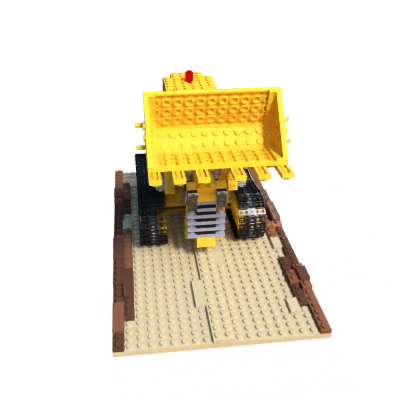
\includegraphics[width=0.3\textwidth]{picture/9.png}
    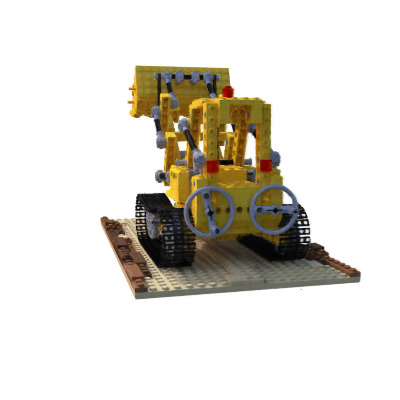
\includegraphics[width=0.3\textwidth]{picture/10.png}
    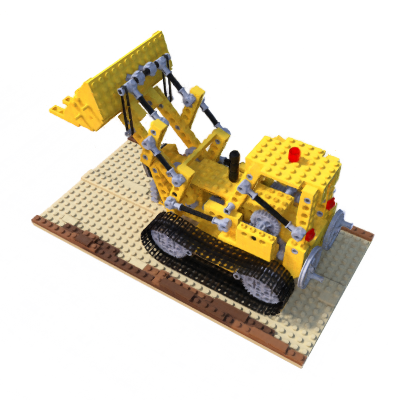
\includegraphics[width=0.3\textwidth]{picture/11.png}
    \caption{NeRF Pytorch模型的训练结果}
\end{figure}
\makespace
\section{NeRF Studio}
\subsection{模型简介}
\textbf{NeRF Studio}是一个基于\textbf{NeRF}的三维重建工具,\textbf{NeRFStudio} 提供了一个图形用户界面,帮助
用户更轻松地使用 \textbf{NeRF} 模型,包括处理视频数据以及生成点云、网格和渲染视频等操作。\textbf{NeRF Studio}
整合了大量\textbf{github}上的开源项目的\textbf{NeRF}模型,使得用户可以更加方便的使用\textbf{NeRF}模型。以下
是一些 \textbf{NeRF Studio} 中包含的知名\textbf{NeRF模型}:
\begin{itemize}
    \item 原始 NeRF:基础的神经辐射场模型。
    \item Instant-NGP:来自 NVIDIA 的快速 NeRF 训练方法。
    \item Nerfacto:NeRFStudio 的默认方法,结合了多个改进。
    \item Mip-NeRF:处理多尺度问题的 NeRF 变体。
    \item TensoRF:用于快速重建的张量分解方法。
    \item LERF: 结合语言和视觉信息的 NeRF 模型。
    \item K-Planes:基于平面的 NeRF 表示方法。
\end{itemize}
\subsection{模型环境配置}
\noindent 于CUDA 12.2 基础下:
\begin{itemize}
    \item Python = 3.11.7
    \item cudatoolkit = 12.1.0
    \item torch = 2.3.0
    \item torchaudio = 2.3.0
    \item torchvision = 0.18.1
\end{itemize}
然后还需配置\textbf{ninja}与\textbf{tiny-cuda},可使用以下命令进行安装:
\begin{lstlisting}[language=bash]
    pip install ninja git+https://github.com/NVlabs/tiny-cuda-nn/
\end{lstlisting}

\indent
如果两个一起安装出现问题,也可以分开安装。接下来可以直接在终端中输入以下命令进行安装\textbf{NeRF Studio}:
\begin{lstlisting}[language=bash]
    pip install nerfstudio
\end{lstlisting}

\indent
如果想获取最新版本的\textbf{NeRF Studio},可以在\textbf{github}上找到\textbf{NeRF Studio}的源代码,
然后在终端中输入命令进行安装,如下:
\begin{lstlisting}[language=bash]
    git clone https://github.com/nerfstudio-project/nerfstudio.git
    cd nerfstudio
    pip install -e .
\end{lstlisting}

\indent
完成即安装成功。

\subsection{预设数据训练}
\hypertarget{6.3}{}
\subsubsection{数据准备}
在项目\textbf{github}上有链接可以前往\textbf{google drive}下载预设数据,下载后将数据放入到任意文件夹中
(因为NeRF Studio是直接下载在电脑上的,所以不用放入到NeRF Studio文件夹中),然后在终端中输入:
\begin{lstlisting}[language=bash]
    ns-train \{想要使用的nerf模型\} --data \{输入文件相对坐标\}
\end{lstlisting}

\indent
命令进行训练。训练时可以通过终端上显示的网址进入到网页中查看训练的进度。
\subsubsection{训练输出}
训练完成后会训练时的位置上生成一个\textbf{outputs文件夹},outputs文件夹中会包含所有训练时使用过的输入文件名。
进入以输入文件名为名字文件后会出现该输入文件使用过的训练模型。进入以模型命名的文件后会出现以不同
时间进行命名的文件,文件里包含了文件名上时间的训练结果,里面主要包含\textbf{配置文件}(config.yml)。
\subsubsection{可视化}
在训练时便可以通过终端上出现的网页查看训练的进度,并可以看到训练的效果。如果在训练完成后想要查看训练的效果,可以在终端中输入:
\begin{lstlisting}[language=bash]
    ns-viewer --load-config {配置文件位置/config.yml}
\end{lstlisting}

\indent
然后便可以在终端上的网页中查看训练的效果。

\subsubsection{点云和mesh图的生成}
\textbf{点云图}和\textbf{mesh图}的生成都会通过\textbf{ns-export}命令进行,只是在命令后面加上不同的参数即可。
但具体使用时需要输入的参数太多,不建议自己去配置和输入。在训练时给出的网页上,进入后有边会有\textbf{Control}、
\textbf{Render}、\textbf{Export}三个板块,如下图:
\begin{figure}[H]
    \hypertarget{6-1}
    \centering
    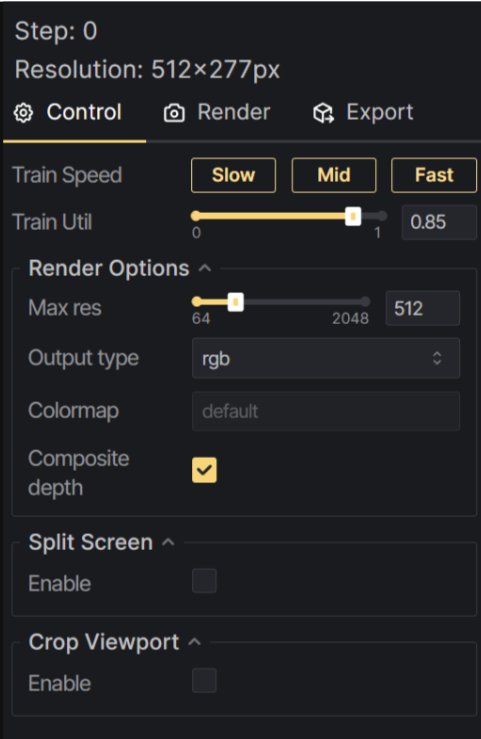
\includegraphics[width=0.5\textwidth]{picture/12.png}
    \caption{NeRF Studio的网页界面的一部分}
\end{figure}

\indent
点击进入\textbf{Export}界面,在{Export}下会有\textbf{Point Cloud}和\textbf{Mesh}两个按钮,最下方有一个\textbf{Generate Command}按钮
,点击后会出现一个命令,将这个命令复制到终端中运行即可生成点云或mesh图。在点击\textbf{Generate Command}按钮前建议先勾选
\textbf{Crop}按钮,点击后左侧的训练界面中会裁剪掉非主体的部分,在输出点云或mesh图时也会同样裁剪掉。实际尝试使用时如果没有勾选
\textbf{Crop}按钮,输出的点云或mesh图会非常的差。如下图:
\begin{figure}[H]
    \centering
    \resizebox{0.4\textwidth}{0.25\textwidth}{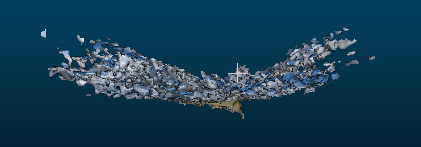
\includegraphics{picture/13.png}}
    \hspace{1cm} % 调整两张图片之间的水平间距
    \resizebox{0.4\textwidth}{0.25\textwidth}{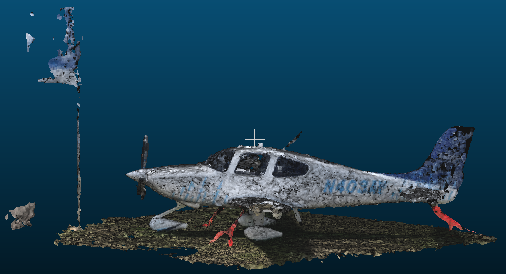
\includegraphics{picture/14.png}}
    \caption{左图为未勾选\textbf{Crop}按钮后的输出,右图为勾选\textbf{Crop}按钮后的输出}
\end{figure}
\subsubsection{渲染视频}
渲染视频是通过\textbf{ns-render}命令进行,与点云和和mesh图的生成一样,也需要在后面加上不同的参数,且也可以在训练的网页上
直接生成命令。在训练网页(如图\hyperlink{6-1}{6-1}所示)中点击\textbf{Render}板块,最下方有一个\textbf
{Generate Command}按钮,点击后会出现一个命令,将这个命令复制到终端中运行正常的话应该就可以得到渲染视频。\\

\indent
但我自己在最开始实际使用的时候发生了报错,在经过解读代码后发现是因为预设数据中的\textbf{camera\_path.json}文件中的
\textbf{camera\_path}为空。为了解决这个问题在经过查找资料后发现解决办法:
\begin{itemize}
    \item 在终端输入:
    \begin{lstlisting}[language=bash]
    ns-export cameras --load-config {配置文件位置/config.yml} 
    --output-dir poses
    \end{lstlisting}
    \item 运行结束后在输出文件夹中会生成\textbf{transforms\_train.json}和\\
    \textbf{transforms\_val.json}两个文件。
    \item 需要将这两个视频转换成\textbf{camera\_path.json}文件,我使用了以下python代码:
    \begin{lstlisting}[language=python]
import json
import numpy as np
from pathlib import Path

def ind(c2w):
if len(c2w) == 3:
c2w += [[0, 0, 0, 1]]
return c2w

train_transforms = json.loads(
    open('poses/transforms_train.json').read()
)
eval_transforms = json.loads(
    open('poses/transforms_eval.json').read()
)
transforms = train_transforms + eval_transforms
print(transforms)

out = {
'camera_type': 'perspective',
'render_height': 1080,
'render_width': 1920,
'seconds': len(transforms),
'camera_path': [
{'camera_to_world': ind(pose['transform']), 'fov': 50, 
'aspect': 1, 'file_path': pose['file_path']}
for pose in transforms
]
}

outstr = json.dumps(out, indent=4)
with open('camera_path.json', mode='w') as f:
f.write(outstr)
\end{lstlisting}
然后再终端中运行此python代码,即可生成\textbf{camera\_path.json}文件。
\item 最后将原文件夹中的\textbf{camera\_path.json}文件替换成新生成的\textbf{camera\_path.json}文件,再次运行网页中生成的
\textbf{ns-render}命令即可得到渲染视频。
\end{itemize}
\subsection{制作数据进行训练}
\subsubsection{数据准备}
选择了我钥匙上的一个小挂件,绕其周围拍摄了一圈,拍摄时需要注意相机与物体之间的距离要尽量保持一致。拍摄完成后将图片放入到一个文件夹中,为读取
相机做准备。
\subsubsection{数据处理}
在NeRF Studio中有一个可以处理数据的工具,可以将图片和视频通过Colmap处理成需要的数据。使用方式及在终端中输入:
\begin{center}
    ns-process-data \{images或者video\} --data \{输入文件相对坐标\} --output-dir \{输出文件相对坐标\}
\end{center}
在我的训练中使用此工具是从视频中仅匹配成功两张照片,所以没有使用这种方法。另外一种处理数据的方法是通过\textbf{
Colmap}(详情见\hyperlink{section 7}{第7章Colmap}),这种方法会比前一种方法复杂一点。首先打开\textbf{Colmap}
软件,在Colmap软件上方点击\textbf{Automatic Reconstruction}。在\textbf{Workspace folder}中选择想要输出
的文件夹,然后在\textbf{Image folder}中选择存放图片的文件夹,接着在\textbf{Data type}中选择对应的数据类型,
最后点击\textbf{Run}即可,随后会在\textbf{Workspace folder}中生成一些文件夹,里面包含了处理后的数据。但还是
会缺少一些\textbf{NeRF Studio}需要的文件,所以需要通过一些其他操作去生成。首先要回到\textbf{Colmap}软件中,在
没有关闭之前的数据的情况下,点击\textbf{File},然后点击\textbf{Export model as text},在弹出的窗口中选择
\textbf{Export cameras}。这样就会在输出文件夹中生成一个\textbf{colmap\_txt}文件夹,里面会包含
\textbf{cameras.txt},\textbf{images.txt},\textbf{points3D.txt},和\textbf{project.ini}四个文件。
然后需要去网上下载一个\textbf{colmap2nerf.py}文件,将这个文件放到和\textbf{colmap\_txt}文件夹同级目录下,
然后在终端中运行\textbf{colmap2nerf.py}文件,即可得到\textbf{transform.json}文件。最后运行\textbf{ns-train},
并将\textbf{Colmap}使用时选择的\textbf{Workspace folder}文件夹为\textbf{--data}的参数,即可开始训练。
\subsubsection{数据训练和输出}
数据训练和输出的方法与预设数据训练和输出的方法一样详情见\hyperlink{6.3}{6.3}。
\subsubsection{自制数据训练结果}
点云图:
\begin{figure}[H]
    \centering
    \resizebox{0.3\textwidth}{0.45\textwidth}{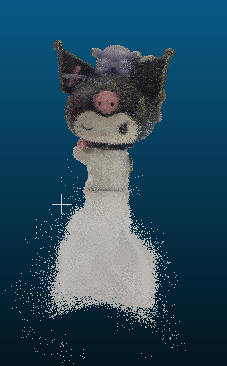
\includegraphics{picture/15.png}}
    \hspace{1cm} % 调整两张图片之间的水平间距
    \resizebox{0.3\textwidth}{0.45\textwidth}{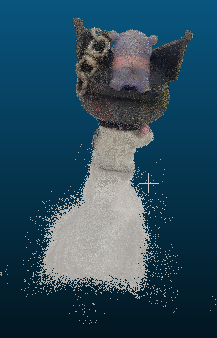
\includegraphics{picture/16.png}}
    \caption{点云输出结果}
\end{figure}
mesh图:
\begin{figure}[H]
    \centering
    \resizebox{0.3\textwidth}{0.45\textwidth}{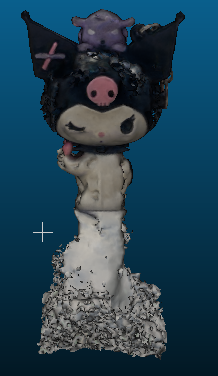
\includegraphics{picture/17.png}}
    \hspace{1cm} % 调整两张图片之间的水平间距
    \resizebox{0.3\textwidth}{0.45\textwidth}{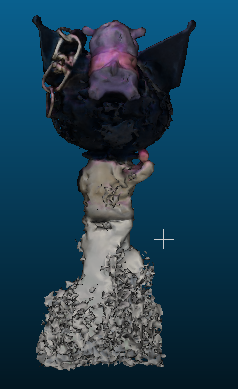
\includegraphics{picture/18.png}}
    \caption{mesh输出结果}
\end{figure}

\subsubsection{航拍数据训练结果}
点云图:
\begin{figure}[H]
    \centering
    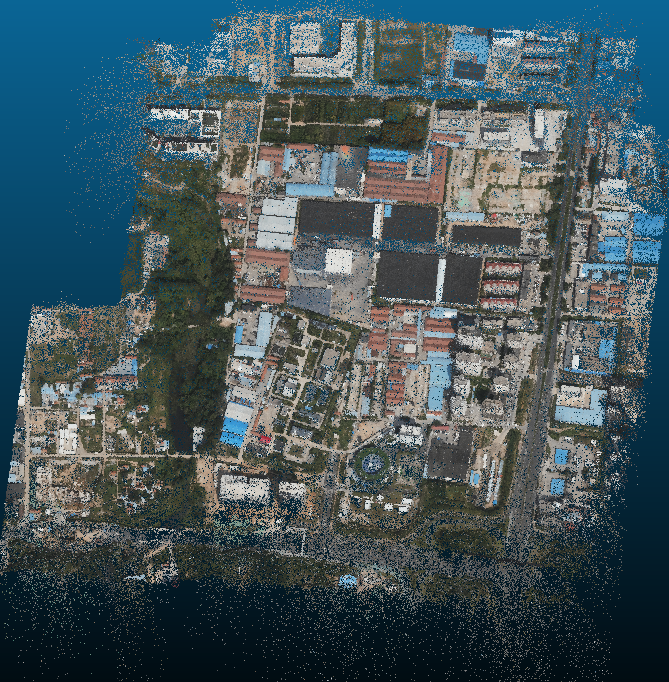
\includegraphics[width=0.8\textwidth]{picture/20.png}
    \caption{点云输出结果}
\end{figure}
\makespace
mesh图:
\begin{figure}[H]
    \centering
    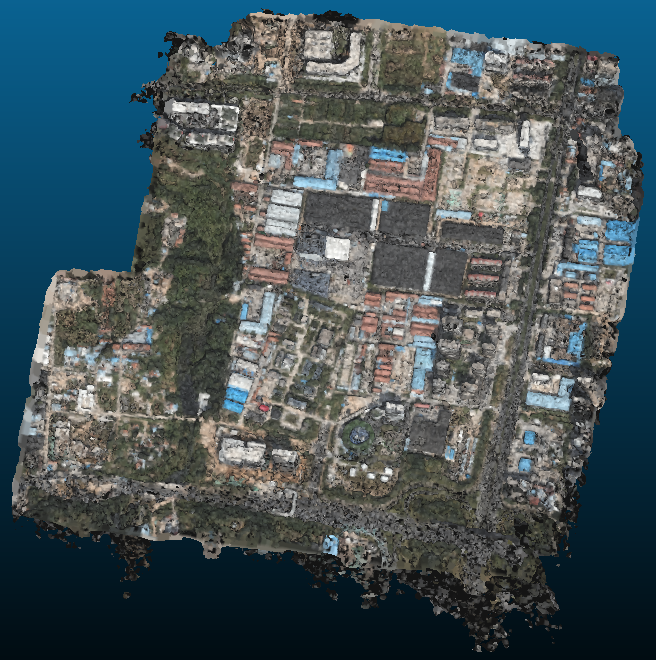
\includegraphics[width=0.8\textwidth]{picture/19.png}
    \caption{mesh输出结果}
\end{figure}

\makespace
\section{Colmap}
\hypertarget{section 7}{}
\subsection{Colmap简介}
\textbf{Colmap}是一个基于\textbf{SfM}(Structure from Motion)和\textbf{MVS}(Multi-View Stereo)的开源软件,
用于从图像序列中重建稀疏或密集的三维模型。\textbf{Colmap}支持多种输入数据类型,包括图像、视频、点云和深度图。\textbf{Colmap}
还支持多种输出数据类型,包括稀疏点云、稠密点云、网格、相机参数、深度图和语义分割等。Colmap的主要功能包括:
\begin{itemize}
    \item 从图像序列中重建稀疏或密集的三维模型
    \item 从视频序列中重建稀疏或密集的三维模型
    \item 从点云中重建稠密的三维模型
    \item 从深度图中重建稠密的三维模型
    \item 从图像中重建稠密的三维模型
    \item 从图像中重建语义分割
\end{itemize}
\subsection{Colmap下载}
官网下载链接:\url{https://colmap.github.io/install.html},根据自己的操作系统进入不同的页面,再根据页面中的步骤下载
即可。\\
\subsection{通过视频或图片生成点云}
在\textbf{Colmap}界面中(如图 7-1),点击\textbf{Reconstruction}:
\begin{figure}[H]
    \centering
    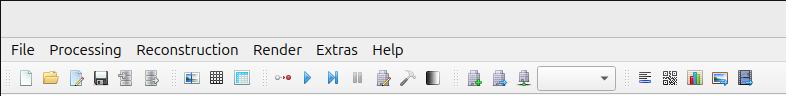
\includegraphics[width=0.8\textwidth]{picture/21.png}
    \caption{Colmap界面}
\end{figure}
\indent
然后点击\textbf{Automatic Reconstruction}。随即将会跳出新界面(如图 7-2),在\textbf{Workspace folder}中选择想要输出的文件夹,
在\textbf{Image folder}中选择存放图片的文件夹,接着在\textbf{Data type}中选择对应的数据类型(通常为
\textbf{Individual images}或\textbf{Video frames}),最后点击\textbf{Run}即可,随后会在
\textbf{Workspace folder}中生成一些文件夹,里面包含了处理后的数据。
\begin{figure}[H]
    \centering
    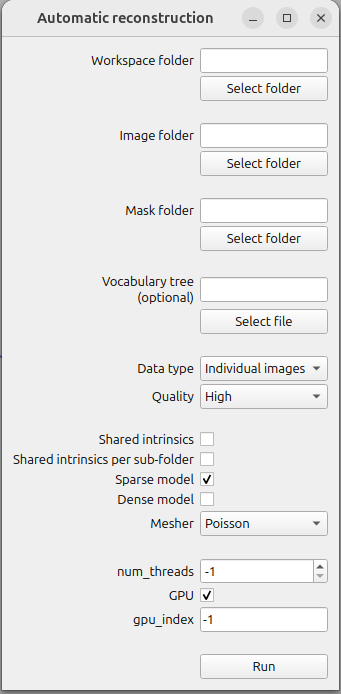
\includegraphics[width=0.5\textwidth]{picture/22.png}
    \caption{Automatic Reconstruction界面}
\end{figure}

\makespace
\hypertarget{SIFT}{}
\subsection{SIFT算法}
\subsubsection{SIFT算法简介}
\textbf{SIFT}(Scale-Invariant Feature Transform)是一种用于图像处理的算法,主要用于检测和描述图像中的局部特征。SIFT算法
的主要步骤包括:
\begin{itemize}
    \item 构建高斯金字塔(Gaussian Pyramid)
    \item 构造高斯差分金字塔(Difference of Gaussian Pyramid)
    \item 关键点检测与定位
    \item 关键点方向分配
    \item 关键点生成特征描述
\end{itemize}
\indent
SIFT算法的主要特点是对图像的尺度、旋转和亮度变化具有不变性,因此在图像配准、目标识别和三维重建等领域有着广泛的应用。

\subsubsection{背景与历史}
SIFT(Scale-Invariant Feature Transform)算法由 Univeristy of British Columbia(UBC)的David Lowe教授在1999年提出,
是图像处理和计算机视觉领域的一项关键技术。该算法专门设计用于检测和描述图像中的局部特征,同时保持对图像尺度、
旋转和亮度变化的不变性。这种不变性使得SIFT算法在图像配准、目标识别和三维重建等多个领域中得到了广泛应用。
SIFT算法的核心优势在于其对图像尺度、旋转和亮度变化的鲁棒性,这为图像分析任务提供了强大的支持。算法的流程包括几个关键步骤:
\begin{itemize}
    \item 尺度空间极值检测以识别潜在的关键点
    \item 精确的关键点定位以提高检测的准确性
    \item 关键点的方向确定,确保特征描述的一致性
    \item 关键点描述的生成,为后续的图像匹配和识别任务提供特征向量
\end{itemize}
\indent
然而,SIFT算法也存在一些局限性。主要缺点是其相对较高的计算复杂度,这要求较为强大的计算资源来处理大规模图像数据集。
尽管如此,SIFT算法的高效性和鲁棒性(Robustness)\footnote{鲁棒性是指系统在面对异常情况时的稳定性和可靠性,即系统
在面对异常情况时能够保持正常的运行状态,不会因为异常情况而崩溃或出现错误。}使得其在图像处理和计算机视觉领域
仍然具有重要的地位。尽管SIFT算法已经有20多年的历史,但其在图像特征提取和匹配方面的优势仍然被广泛认可,
并且在许多领域中仍然是一种重要的技术。
\subsubsection{SIFT算法原理}
\noindent
第一步:高斯金字塔的构建。\\
\indent
将原始图像作为高斯金字塔的第一层(即最底层),不进行任何修改。对每一层图像进行\textbf{高斯滤波}(Gaussian Blur,公式7-1)
\footnote{高斯滤波是一种线性平滑滤波器,它使用高斯函数作为卷积核。高斯滤波器的卷积核是一个二维的高斯函数,可以有效
的去除图像中的高斯噪声。}。
\hypertarget{公式7-1}{}
\begin{equation}
    \begin{aligned}
        G(x,y,\sigma) &= \frac{1}{2\pi\sigma^2}e^{-\frac{x^2+y^2}{2\sigma^2}}\\
        L(x,y,\sigma) &= G(x,y,\sigma) * I(x,y)\\
    \end{aligned}
\end{equation}
\indent
其中:
\begin{itemize}
    \item L 表示高斯金字塔(Gaussian Pyramid)中的一个层级。高斯金字塔是通过对原始图像进行重复的高斯模糊和降采样操作生成的图像序列。L 可以表示金字塔中的某一层,也就是在特定尺度下的图像。
    \item G 表示高斯滤波器(Gaussian Filter)。在 SIFT 算法中,图像在构建高斯金字塔时会通过应用高斯滤波器进行模糊处理,以减少图像的高频信息。G 是这个滤波器的表示。
    \item I 表示图像的梯度(Gradient)。在 SIFT 中,用于计算关键点的主方向时,会计算图像的梯度信息,以便确定关键点的旋转不变性。梯度信息对于描述图像的局部特征方向是至关重要的。
\end{itemize}

\indent
然后对对经过高斯滤波的图像进行\textbf{降采样}(Downsampling)\footnote{降采样是一种减小图像尺寸的方法,通过减少
图像的像素数量,可以减小图像的尺寸。降采样通常使用像素平均或其他插值方法来缩小图像,生成下一层的图像},生成下一层的
图像。重复的进行高斯滤波和降采样,直到达到所需的金字塔层数或者图像尺寸不再变化。\\
\indent
通过这个过程,原始图像被分解成一系列不同尺度的图像,每个尺度上的图像都是通过对前一个尺度图像进行高斯模糊和降采样得到的。
这样的分解使得图像在不同尺度上都能够被有效地表示,从而为诸如特征检测、图像配准和目标识别等任务提供了基础。最后的
高斯金字塔如下图所示:(图7-3)
\begin{figure}[H]
    \centering
    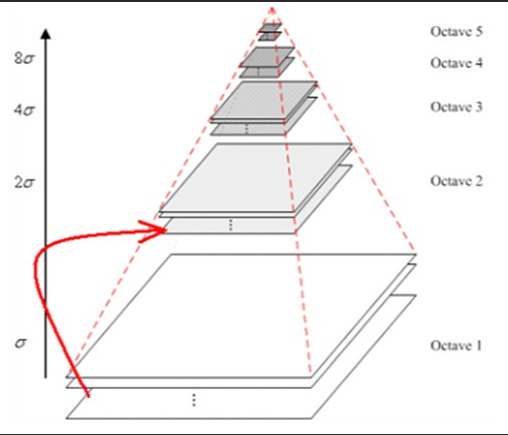
\includegraphics[width=0.8\textwidth]{picture/23.png}
    \caption{高斯金字塔}
\end{figure}
\noindent
第二步:构造\textbf{高斯差分金字塔}(DOG,difference of gaussian)\\
\indent
在构建高斯金字塔的基础上,通过对相邻两层图像进行减法运算,得到一系列的高斯差分图像。高斯差分图像的构建过程如下:(公式7-2)
\begin{equation}
    \begin{aligned}
        D(x,y,\sigma) &= (G(x,y,k\sigma) - G(x,y,\sigma)) * I(x,y)\\
    \end{aligned}
\end{equation}

\indent
其中$G(x,y,\sigma)$和$I(x,y)$的含义与\hyperlink{公式7-1}{公式7-1}中相同,k是一个常数,通常取值为$\sqrt{2}$, 
$D(x,y,\sigma)$ 表示图像的差分(Difference),表示两个高斯模糊图像之间的差异。通过这个过程,
我们可以得到一系列的高斯差分图像。\\ \\
\indent
过程如下图:(图7-4)
\begin{figure}[H]
    \centering
    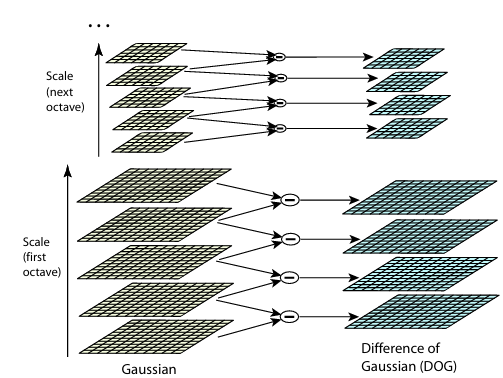
\includegraphics[width=0.8\textwidth]{picture/24.png}
    \caption{高斯差分金字塔}
\end{figure}
\noindent
第三步:关键点的检测\\
\indent
在高斯差分金字塔中,我们可以通过检测\textbf{局部极值点}\footnote{局部极值点是指在图像中的一个像素点,其值比周围像素点的值
都要大或者都要小。}来确定关键点。在每个\textbf{Octave}(八度)\footnote{Octave是高斯金字塔的组,每个Octave包含一系列
的高斯模糊图像和高斯差分图像。}中,从第二层开始对每个像素点进行检测,判断其是否为局部极值点,及是否为周围26个像素点(
包括上下层分别9个点和同层的8个像素点)中的最大值或最小值。那么这个点就是一个局部极值点。\\
\indent
接下来我们需要对关键点的位置进行精确定位,首先对每一个检测到的极值点$X(x,y,z)$进行三元二阶泰勒展开式(Taylor Expansion)
\footnote{泰勒展开式是一种用多项式来逼近函数的方法,通过泰勒展开式可以将一个函数在某一点的邻域内用一个多项式来逼近。}。
公式如下(公式7-3):
\begin{equation}
    \begin{aligned}
        D(X) &= D + \frac{\partial D^T}{\partial X}X + \frac{1}{2}X^T\frac{\partial^2D}{\partial X^2}X\\
    \end{aligned}
\end{equation}

\indent
其中$D$是极值点的值,$\frac{\partial D^T}{\partial X}$是梯度向量,$\frac{\partial^2D}{\partial X^2}$是Hessian矩阵。
通过求解这个二次曲面的极值点,可以得到比原始DoG图像中检测到的更精确的关键点位置。这涉及到计算一阶导数为零的条件,并使用二阶导
数来确定极值点的稳定性。
\\
\indent
我们在图像中找到的局部极值点可能只是近似的极值点,真实的极值点可能位于局部极值点周围的某个位置。这是因为图像中的噪声、
图像变化的不连续性以及离散化的像素值等因素可能会导致局部极值点的位置不够准确。为了解决这个问题,我们使用泰勒展开来对极值点
周围的像素区域进行近似描述。通过泰勒展开,我们可以获得一个多项式,可以更准确地描述极值点周围像素的强度变化。然后,我们可以
通过迭代优化来调整多项式的参数,以使其在该区域内的近似误差最小化,从而找到更准确的极值点位置。\\
\\
第四步:关键点方向分配\\
\indent
在确定了关键点的位置之后,我们需要确定关键点的主方向。这是为了使得关键点对于旋转的变化具有不变性。在确定关键点的主方向时,
我们首先计算关键点周围的梯度信息,然后通过对梯度信息进行加权,计算出关键点的主方向。\\
\indent
在计算关键点的主方向时,我们首先将关键点半径为$1.5\sigma$的邻域作为\textbf{方向直方图}(orientation histogram)
\footnote{方向直方图是一种用来描述数据中各个值的分布情况的图表。在SIFT算法中,我们将关键点周围的梯度方向分布到方向直方图中,
然后通过统计直方图中的梯度方向分布,找到最大的峰值,这个峰值对应的方向就是关键点的主方向。}。在方向直方图中
划分$36$个方向区间,每个区间为$10$度。然后,我们对范围内的每个像素点计算其梯度方向,然后将梯度幅值加权到相应的方向区间中。
梯度方向计算公式如下:(公式7-4)\\
\begin{equation}
    \begin{aligned}
        m(x,y) &= \sqrt{L(x+1,y) - L(x-1,y)^2 + L(x,y+1) - L(x,y-1)^2}\\
        \theta(x,y) &= tan^{-1}(\frac{L(x,y+1) - L(x,y-1)}{L(x+1,y) - L(x-1,y)})\\
    \end{aligned}
\end{equation}

其中,L(x,y)为当前特征点,m(x,y)表示梯度幅值,$\theta(x,y)$表示梯度方向。\\

\indent
最后,我们统计方向直方图中的梯度方向分布,找到最大的峰值,这个峰值对应的方向就是关键点的主方向。\\
\\
第五步:生成特征描述\\
\indent
在确定了关键点的位置和方向之后,我们需要生成关键点的特征描述。这个描述是一个向量,用来描述关键点周围的图像区域。
在 SIFT 算法中,我们首先将关键点周围的图像区域划分为$d\times d$个子区域,每个子区域划分为8个方向(每个方向45度)。
每个子区域大小为m$\sigma$$\times$m$\sigma$。(原论文中使用d=4, m=3)
如下图(图7-5):\\
\begin{figure}[H]
    \centering
    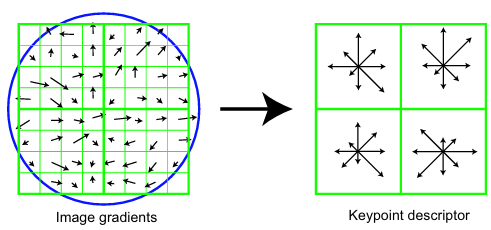
\includegraphics[width=0.8\textwidth]{picture/25.png}
    \caption{特征描述}
\end{figure}

\indent
接着旋转特征描述,和整个图的主方向的水平x轴平行。然后计算旋转后领域范围内像素的梯度方向和幅值,最后使用
\textbf{高斯加权}(Gaussian Weighting)\footnote{高斯加权是一种用高斯函数对数据进行加权的方法,通过高斯加权,
可以使得数据在中心附近的权重更大,而在边缘附近的权重更小。}得到了关键点的特征描述。最后将特征描述归一化,以减少光照、
尺度和旋转等因素的影响。\\

\subsubsection{SIFT算法在Colmap中的应用}
\indent
\textbf{Colmap}中的\textbf{SFM}(Structure from Motion)和\textbf{MVS}(Multi-View Stereo)算法中都使用了
\textbf{SIFT}算法。在\textbf{SFM}算法中,\textbf{SIFT}算法用于检测和描述图像中的局部特征,以便在多个图像之间
进行特征匹配。在\textbf{MVS}算法中,\textbf{SIFT}算法用于检测和描述图像中的局部特征,以便在多个图像之间进行
特征匹配。通过特征匹配,我们可以找到多个图像之间的对应关系,从而可以计算出相机的位姿和三维点的位置。\\
\makespace
\subsection{SFM}
\subsubsection{SFM简介}
\textbf{SFM}(Structure from Motion)是一种用于从图像序列中重建三维场景的技术。SFM的基本思想是利用多个图像
中的共同特征点,通过匹配这些特征点并估计相机的位置和姿态,来重建三维场景。SFM算法的主要步骤包括:
\begin{itemize}
    \item 特征提取:从多个图像中提取共同的特征点
    \item 特征匹配:对提取的特征点进行匹配,找到多个图像之间的对应关系
    \item 相机定位:通过特征匹配,估计相机的位置和姿态
    \item 三维重建:通过相机的位置和姿态,计算出三维场景的结构
\end{itemize}
\indent
其中特征提取便是通过上文中的\textbf{\hyperlink{SIFT}{SIFT}}算法来实现的。SFM算法在计算机视觉、机器人技术、
增强现实等领域有着广泛的应用,是一种重要的三维重建技术。
\subsubsection{SFM算法原理}
\indent
在通过\textbf{SIFT}算法提取了图像中的特征点之后,我们需要对这些特征点进行匹配。首先我们通过比较不同图像中
特征点的描述符来寻找匹配点。通常,我们会采用最近邻匹配策略,为每个特征点找到其在其他图像中最相似的对应点。
为了提高匹配的准确性,我们还会使用距离比值测试来过滤掉那些不够显著的匹配。\\
\indent
此外,\textbf{RANSAC}算法在这一步骤中发挥着重要作用,它通过随机选择的匹配点对来估计模型参数,并排除那些
与模型不一致的异常值,从而确保最终匹配结果的鲁棒性。最后,通过这一系列的匹配策略和优化技术,我们能够得到
一组可靠的特征点匹配。\\
\indent
在通过SIFT算法成功提取并匹配图像中的特征点之后,我们接下来的任务是通过这些特征点匹配来估计相机的位置和姿态。
这一关键步骤通常采用\textbf{PnP}(Perspective n Point)\footnote{PnP算法是一种用于估计相机位姿的技
术,通过已知的三维点和它们在图像上的对应点,来求解相机的旋转矩阵和平移向量。}算法来实现。PnP算法通过最小化
重投影误差来求解相机的旋转矩阵和平移向量,从而估计相机的位姿。为了提高求解的准确性,我们通常结合
\textbf{RANSAC}算法来排除异常值和错误匹配,确保我们获得准确的相机位姿估计。\\

一旦相机的姿态被准确估计,我们便可以利用这些信息,结合特征点匹配,通过三角测量的方法计算出三维空间中点的精确位置,
从而构建起稀疏的三维点云。随后,通过全局优化技术如Bundle Adjustment进一步优化相机位姿和三维点位置,
最小化整个场景的重投影误差。在稀疏重建的基础上,我们还可以采用密集重建技术,通过分析图像的像素级信息来生成更加
精细和完整的三维模型。最后,对生成的三维点云进行必要的后处理,如平滑处理和去噪,以提高重建结果的质量和可用性。
这样,我们就从二维图像中恢复出了三维场景的结构,实现了三维重建的目标,为进一步的应用如虚拟现实、增强现实和
三维打印等打下了坚实的基础。





\makespace
\section*{致谢}
\begin{center}
    { \blackti \fontsize{16.0600pt}{1.25}致 \, 谢}
\end{center}
\addcontentsline{toc}{section}{致\texorpdfstring{ \, }{} 谢}
\myspace{1}
致谢内容。

\makespace
\section*{文献}
\begin{center}
    { \blackti \fontsize{16.0600pt}{1.25}文 \, 献}
\end{center}
\addcontentsline{toc}{section}{文\texorpdfstring{ \, }{} 献}
\myspace{1}
\noindent
Mildenhall, B., Srinivasan, P. P., Tancik, M., Barron, J. T., Ramamoorthi, R., \& Ng, R. (2020). NeRF: 
Representing Scenes as Neural Radiance Fields for View Synthesis. In European Conference on Computer Vision 
(ECCV).\\\\
Lowe, D. G. (1999). Object recognition from local scale-invariant features. International Journal of Computer Vision, 29(2), 91-110.\\\\
Lowe, D. G. (2004). Distinctive image features from scale-invariant keypoints. International Journal of Computer Vision, 60(2), 91-110.\\\\
\end{document}

